\textbf{COLUNI 2023 -- Questão 32}\par\medskip Analise a imagem e o texto a seguir.

\begin{center}\textbf{UFV COMEMORA SUCESSO DE PÚBLICO NA SEMANA DO FAZENDEIRO.}\end{center}

% COLUNI-AUTO-FIGURES-BEGIN
\begin{figure}[htbp]
\centering
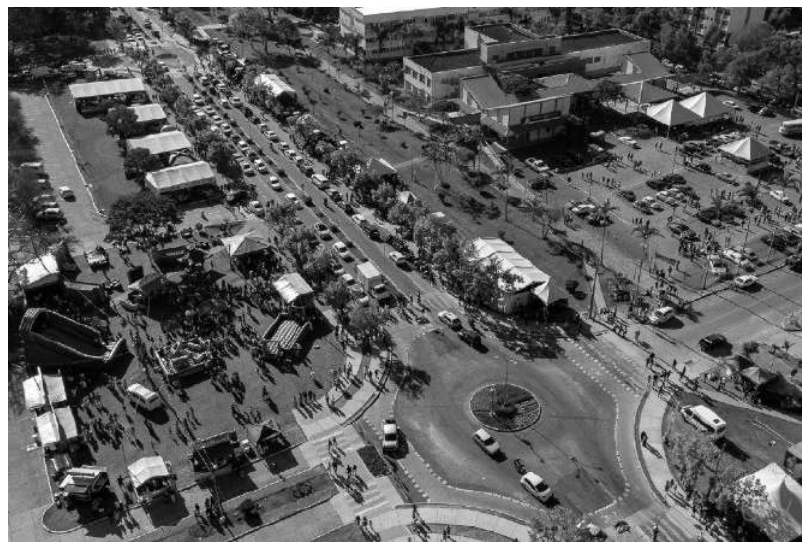
\includegraphics[width=0.95\linewidth]{static/simulados/coluni/figuras/2023/questao-32/figura-1.png}
\end{figure}
% COLUNI-AUTO-FIGURES-END
\begin{center}Evento volta a acontecer presencialmente após dois anos de pausa\end{center}

A Semana do Fazendeiro, o maior evento de extensão da UFV, esteve de volta ao campus Viçosa, com atividades presenciais na semana de 13 a 19 de agosto de 2022. A programação contou com atrações para todas as idades.

Com o tema “Plantar, Cuidar, Florescer: Sonhos, Conquistas, Vidas”, a 92ª Semana do Fazendeiro ofertou 262 oportunidades de capacitação em diversas áreas, como bovinocultura, cafeicultura, controle de pragas, processamento de alimentos e produção artesanal.

Uma das atrações mais visitadas é a mini fazenda [...]. Diversas escolas de Viçosa e região levaram seus alunos para uma visita guiada ao espaço.

\begin{center}Fonte. Jornal Folha da Mata. Viçosa. Ano LIX n. 2778, 18/08/2022, p. 6. (Adaptado)\end{center}

Sobre a Semana do Fazendeiro, que ocorreu no campus da UFV e sobre a agricultura brasileira, é CORRETO afirmar:
\begin{enumerate}
\item É uma atividade agrícola de extensão voltada, exclusivamente, para as pequenas propriedades e seus
      produtores, pois leva-se em consideração a grande quantidade de minifúndios rurais existentes em Minas
      Gerais.
\item É um evento raro, destinado apenas aos fazendeiros que trabalham com a pecuária intensiva, na qual o
      gado é criado confinado, gerando um produto de melhor qualidade e de maior rentabilidade, o que
      favorece a sua exportação.
\item A agricultura praticada no Brasil se encontra dividida entre a familiar, aquela na qual os processos
      produtivos são executados pelos membros de uma família e a patronal, realizada por empresas agrícolas
      e por seus trabalhadores contratados.
\item A modernização agrícola no campo tem favorecido o emprego de um maior número de máquinas e de
      equipamentos, propiciando o aumento da produtividade, principalmente na região Norte, onde o
      desmatamento vem favorecendo a formação de novas propriedades rurais produtivas.
\end{enumerate}
